\documentclass[hidelinks]{ctexart}

\usepackage{van-de-la-illinoise}

\begin{document}

\section{量子力学初步} % (fold)
\label{sec:量子力学初步}

\subsection{实物粒子波动性} % (fold)
\label{sub:实物粒子波动性}

光的粒子性和波动性通过
\[ E = h \nu,\quad \lambda = \frac{h}{p} \]
联系起来. de Broglie指出实物粒子也具有波动性, $\displaystyle \resumath{ \lambda = \frac{h}{p}.}$ 其中$h$为Planck常数, $h=\SI{6.626e-34}{\joule\cdot\second}$.
\par
相对论情形下,
\[ \lambda = \frac{hc}{\sqrt{2m_0 c^2 T}\sqrt{1+T/2m_0c^2}}. \]
非相对论情形下$\displaystyle \lambda = \frac{hc}{\sqrt{2m_0 E}}$.
\begin{sample}
    \begin{ex}
        一个$\SI{100}{\gram}$的子弹以$\SI{100}{\meter\per\second}$的速度运动, 则其de Broglie波长为
        \[ \lambda = \frac{h}{p} = \frac{h}{m_0 v} = \SI{6.63e-35}{\meter}. \]
        一个$\SI{100}{\eV}$电子的de Broglie波长为
        \[ \lambda = \frac{hc}{\sqrt{2m_0c^2T}} = \SI{0.123}{\nano\meter}. \]
    \end{ex}
\end{sample}
氢原子的能态可以通过de Broglie波解释. 为了形成驻波, 对于势阱应有$\displaystyle L = n\cdot \lambda/2$. 对于氢原子,
\[ 2\pi r = n\lambda,\quad \lambda = \frac{2\pi r}{n} = \frac{h}{p} \Rightarrow L = m_e vr = pr = \frac{h}{\lambda} r = \frac{nh}{2\pi r}r = n\hbar. \]
这正是角动量量子化.

\subsubsection{电子晶体衍射实验} % (fold)
\label{ssub:电子晶体衍射实验}

热电子经过加速后会在固体晶格表面发生衍射(无法穿入固体内部). 对于垂直界面入射的情形, 不同入射动能会在不同角度处出现衍射极大. 相干条件
\[ d \sin \theta = n\lambda,\quad n = 1,2,3,\cdots. \]
举例而言, 当电子能量$T = \SI{54}{\eV}$, 有
\[ \lambda = \frac{h}{\sqrt{2mT}} \approx \SI{0.167}{\nano\meter}, \]
和实验的$d\sin\theta$符合.
\begin{figure}[ht]
    \centering
    \incfig{4cm}{CrystSurfRefl}
\end{figure}
\begin{remark}
    参考G.P. Thompson的电子投射金属箔的实验, 电子的单缝/多缝干涉实验, 以及双棱镜实验.
\end{remark}

\paragraph{原子干涉仪} % (fold)
\label{par:原子干涉仪}

通过合并的电子束将基态的氦原子升高至激发态, 便于探测, 可以观察到氦原子的干涉.
\[ T=\SI{295}{\kelvin},\quad E_k = \frac{3}{2}k_BT \approx \SI{0.038}{\eV},\quad \lambda = \frac{hc}{\sqrt{2Mc^2E_k}} \approx \SI{0.073}{\nano\meter}. \]
\begin{remark}
    分子之间也会发生干涉, 例如 \ce{C_{60}}.
\end{remark}

% paragraph 原子干涉仪 (end)

\paragraph{冷原子干涉仪} % (fold)
\label{par:冷原子干涉仪}

对于$T=\SI{100}{\nano\kelvin}$, $\displaystyle E_k = \frac{3}{2}k_BT$更小, $\lambda$在$\SI{}{\micro\meter}$量级, 故更易观察到现象.

\begin{remark}
    双原子分子本身亦可作为一分子尺度干涉, 因为光线入射随机电离两个原子中的一个, 发生Fano-Cohen干涉.
\end{remark}

% paragraph 冷原子干涉仪 (end)

% subsubsection 电子晶体衍射实验 (end)

\subsubsection{波粒二象性} % (fold)
\label{ssub:波粒二象性}

\paragraph{经典子弹双缝} % (fold)
\label{par:经典子弹双缝}

假设单颗子弹的完整性, 任何时刻墙上没有或有且仅有一颗子弹击中, 则射出者射出的单颗子弹的角度与分布概率是确定的, 与射速无关的. 大量射击后,
\[ P_{12} = P_1 + P_2. \]
其中$P_1$是穿过缝I的概率, $P_2$是穿过缝II的概率.

% paragraph 经典子弹双缝 (end)

\paragraph{经典水波的干涉实验} % (fold)
\label{par:经典水波的干涉实验}

遮上缝II, $I_1 = \abs{h_1}^2$, 遮上缝I, $I_2 = \abs{h_2}^2$. 两个缝都打开, 则
\[ I_{12} = \abs{h_1 + h_2}^2 = \abs{h_1}^2 + \abs{h_2}^2 + 2\abs{h_1h_2}\cos\delta \neq I_1 + I_2. \]
故波的干涉存在干涉项.

% paragraph 经典水波的干涉实验 (end)

\paragraph{电子的双缝干涉实验} % (fold)
\label{par:电子的双缝干涉实验}

虽然电子完整, 任何时刻都没有或有且仅有一个电子击中, 且射出电子的角度与分布概率是确定的, 仍然观察到了电子的干涉图样. 从而考虑引入$\phi$, 满足
\[ P_1 = \abs{\phi_1}^2,\quad P_2 = \abs{\phi_2}^2,\quad P_{12} = \abs{\phi_1 + \phi_2}^2. \]
如果在狭缝出跟踪电子的位置, 会有
\[ P'_{12} = P'_1 + P'_2. \]
此时丢失干涉图样.
\par
利用长波光源, 散射时光子对电子的扰动足够小, $p = h/\lambda$. 但是波长长到狭缝间隔的尺度时, 将无法判断电子从哪个狭缝通过.
\par
将电子束入射 \ce{N_2} 分子, 通过探测分子的反冲可得知被电离的原子.

% paragraph 电子的双缝干涉实验 (end)

% subsubsection 波粒二象性 (end)

\subsubsection{不确定关系} % (fold)
\label{ssub:不确定关系}

\begin{figure}[ht]
    \centering
    \incfig{6cm}{SingleG}
\end{figure}
用宽度$d$的单缝确定电子的位置, 为了使其轨迹更精确, $d$应尽可能小, 但此时主极大将变宽. 电子在$d$方向的不确定度$\Delta x \sim d$, 极小值点$d\sin\theta = k\lambda$, 而$\displaystyle \lambda = \frac{h}{p}$. 电子打过狭缝后, 一级主极大$\sin \theta_1 = \lambda/d$, 动量$p_x$在$0\sim p\sin\theta_1$之间. 故$p_x$具有不确定性
\[ \Delta p_x = p\sin\theta_1 = p \frac{\lambda}{d} = p\rec{d}\frac{h}{p} = \frac{h}{d} \sim \frac{h}{\Delta x}. \]
\begin{resume}
    \[ \Delta p_x \Delta x \ge \frac{\hbar}{2},\quad \Delta E\Delta t \ge \frac{\hbar}{2}. \]
\end{resume}
\begin{sample}
    \begin{ex}
        利用不确定关系估算氢原子基态能量.
    \end{ex}
    \begin{solution}
        $\displaystyle E = \frac{p^2}{2m} - \frac{e^2}{4\pi\epsilon_0 r}$. 位置的不确定度$\Delta r \sim r$, $\Delta p \sim p$, 从而由不确定关系,
        \[ r\cdot p = \hbar. \]
        代入得$\displaystyle E = \frac{p^2}{2m} - \frac{e^2p}{4\pi\epsilon_0 \hbar}$. 令其具有极小值,
        \[ p\+_min_ = \frac{me^2}{4\pi\epsilon_0 \hbar}. \]
        相应的
        \[ r = \frac{\hbar}{p\+_min_} = \frac{4\pi\epsilon_0 \hbar^2}{e^2m} = a_0,\quad E\+_min_ = -\frac{e^4m}{2\cdot\pare{4\pi\epsilon_0}^2\hbar^2} = \SI{-13.6}{\eV}. \qedhere \]
    \end{solution}
\end{sample}

\paragraph{能量-时间不确定关系} % (fold)
\label{par:能量_时间不确定关系}

激发态有一定的寿命$\Delta t = \tau$, 能量$E_b$有不确定度$\Delta E = \Gamma$. 则不确定关系表明$\Gamma\tau \sim h$. 通常能级寿命为$\SI{e-8}{\second}\sim\SI{e-9}{\second}$, 相应的宽度为$\SI{e-8}{\eV}\sim \SI{e-7}{\eV}$.

% paragraph 能量_时间不确定关系 (end)

% subsubsection 不确定关系 (end)

% subsection 实物粒子波动性 (end)

\subsection{波函数及其统计解释} % (fold)
\label{sub:波函数及其统计解释}

\subsubsection{波函数的引入} % (fold)
\label{ssub:波函数的引入}

\paragraph{经典波} % (fold)
\label{par:经典波}

弦振动和电磁波都满足形如$\displaystyle \frac{\partial^2 u}{\partial x^2} = \rec{v^2}\frac{\partial^2 u}{\partial t^2}$的方程, 有谐波解$u \propto \cos\pare{kx - \omega t}$.

% paragraph 经典波 (end)

\paragraph{de Broglie波} % (fold)
\label{par:de_broglie波}

不受外力作用时, 动能和动量保持不变, $E = h\nu = \hbar \omega$, $\+vp = \hbar \+vk$. 自由粒子的de Broglie波的波长和频率也是不变的, 是一个平面单色波.
\[ \Psi\pare{\+vr,t} = \Psi_0 e^{i\pare{\+vk\cdot \+vr - \omega t}} = \Psi_0 e^{\frac{i}{\hbar}\pare{\+vp\cdot \+vr - Et}}. \]

% paragraph de_broglie波 (end)

\par
电子本身可视为以波包结构, 波包的大小即电子的大小, 波包的群速度即电子的速度.
\[ \Psi\pare{\+vr,t} = \sum_j \Psi_0 e^{\frac{i}{\hbar}\pare{\+vp_j \cdot \+vr - E_j t}}. \]
可以认为电子的单缝衍射中, 打在屏上$x$点的电子数$\propto$单个电子在$x$点的概率分布. 设电子到达屏幕的波函数为$\Psi\pare{x}$, 类比光的衍射, 衍射条纹强度分布$\abs{\Psi\pare{x}}^2$.
\par
\begin{resume}
    \begin{axiom}[波函数的统计诠释]
        $\abs{\Phi\pare{\+vr,t}}^2\,\rd{\tau}$表示$\+vr$处体积元$\rd{\tau}$内粒子出现的概率.
    \end{axiom}
\end{resume}
在电子的单缝衍射实验中, 电子从缝I通过时波函数记作$\Psi_1$, 从缝II通过时波函数记作$\Psi_2$. 两个缝都打开时, 电子处于叠加态, 概率密度为$\abs{\Psi_1 + \Psi_2}^2$.
\par
若引入光源以探测电子从哪一条缝穿过, 则
\begin{cenum}
    \item 电子I被看到, 则电子塌缩至$P_1 = \abs{\Psi_1\pare{x}}^2$.
    \item 电子II被看到, 则电子塌缩至$P_2 = \abs{\Psi_2\pare{x}}^2$.
    \item 电子没有被看到, 则电子仍然处于两个态的叠加, $P_{12} = \abs{\Psi_1 + \Psi_2}^2$.
\end{cenum}
不同的量子态可以叠加, 若$\curb{\Psi_i}$构成一组基, 则$\sum c_i \Psi_i$构成一波函数.
\par
质量为$m$的自由粒子的波函数为平面单色波,
\[ \displaystyle \Psi\pare{\+vr,t} = \Psi_0 \exp \curb{\frac{\hbar}{i}\pare{\+vp\cdot \+vr - Et}}, \]
求时间求偏微分,
\[ \+DtD\Psi = -\frac{i}{\hbar} E \Psi. \]
对位置求偏微分,
\[ \+D{x^2}D\Psi = -\pare{p_x^2}{\hbar^2}\Psi \Rightarrow \laplacian \Psi = -\frac{p^2}{\hbar^2}\Psi. \]
由此得到动能算符.
\begin{resume}
    \vspace{-\baselineskip}
    \begin{flalign*}
        & \text{Schr\"odinger方程} && i\hbar \+DtD\Psi = \brac{-\frac{\hbar^2}{2m}\laplacian + V\pare{\+vr,t}} \Psi. &&
    \end{flalign*}
\end{resume}

% subsubsection 波函数的引入 (end)

% subsection 波函数及其统计解释 (end)

\subsection{\texorpdfstring{Schr\"odinger}{Schrodinger}方程} % (fold)
\label{sub:schrodinger方程}

\subsubsection{概率密度守恒} % (fold)
\label{ssub:概率密度守恒}

概率密度$\rho\pare{\+vr,t} = \abs{\Psi\pare{\+vr,t}}^2$, 则
\begin{align*}
    \+DtD\rho &= \Psi^*\+DtD{\Psi} + \Psi \+DtD{\Psi^*} = \rec{i\hbar}\cdot \pare{-\frac{\hbar^2}{2m}}\pare{\Psi^* \laplacian \Psi - \Psi \laplacian \Psi^*}.
\end{align*}
从而
\[ \+DtD\rho + \div \+vj\pare{\+vr,t} = 0,\quad \+vj = \frac{\hbar}{2mi}\pare{\Psi^*\grad \Psi - \Psi \grad \Psi^*}. \]

% subsubsection 概率密度守恒 (end)

\subsubsection{波函数的标准条件} % (fold)
\label{ssub:波函数的标准条件}

\begin{cenum}
    \item 平方可积: 满足归一化条件, $\displaystyle \iiint_V \Psi^*\Psi \,\rd{\tau} = 1$.
    \item 有限, 单值, 连续且在$V\pare{\+vr}$连续时$\Psi$的一阶导数应当连续.
    \item 叠加态原理: 若$\Psi_1,\Psi_2,\cdots$满足Schr\"odinger方程, 则其线性组合
    \[ \Psi = c_1\Psi_1 + c_2\Psi_2 + \cdots \]
    也满足Schr\"odinger方程, 也是描述粒子的波函数.
\end{cenum}

% subsubsection 波函数的标准条件 (end)

\subsubsection{定态\texorpdfstring{Schr\"odinger}{Schrodinger}方程} % (fold)
\label{ssub:定态schrodinger方程}

在类氢原子中, $\displaystyle V\pare{\+vr} = -\frac{Ze^2}{4\pi\epsilon_0r}$, 故
\[ i\hbar \+DtD\Psi = \hat{H} \Psi \xLongrightarrow{\Psi\pare{\+vr,t} = u\pare{\+vr}f\pare{t}} \begin{cases}
    \displaystyle \+dtd{f\pare{t}} = \frac{E}{i\hbar}f\pare{t} \Rightarrow f\pare{t} = C\exp\pare{-\frac{i}{\hbar}Et}. \\[1em]
    \displaystyle \pare{-\frac{\hbar^2}{2m}\laplacian + V\pare{\+vr}} u\pare{\+vr} = Eu\pare{\+vr}.
\end{cases} \]
总的波函数为$\displaystyle \Psi\pare{\+vr,t} = u\pare{\+vr} \exp\pare{-\frac{i}{\hbar}Et}.$

\paragraph{定态} % (fold)
\label{par:定态}

定态下总能量$E=T+V$不随时间变化, 粒子概率的分布不随时间变化,
\[ \rho\pare{\+vr,t} = \abs{\Psi\pare{\+vr,t}}^2 = \abs{u\pare{\+vr}\exp\pare{-\frac{i}{\hbar} Et}}^2 = \abs{u\pare{\+vr}}^2. \]
定态满足Schr\"odinger方程
\[ \resumath{\pare{-\frac{\hbar^2}{2m} \laplacian + V\pare{\+vr}} u\pare{\+vr} = Eu\pare{\+vr}.} \]

% paragraph 定态 (end)

% subsubsection 定态schrodinger方程 (end)

\subsubsection{一维定态问题} % (fold)
\label{ssub:一维定态问题}

\begin{sample}
    \begin{ex}
        无限深方势阱中, $\displaystyle V\pare{x} = \begin{cases}
            0, & 0\le x\le a,\\
            \infty, & x < 0\quad \mathrm{or} \quad x>a.
        \end{cases}$
    \end{ex}
    \begin{solution}
        在势阱外, 必定有$u = 0$. 势阱内应有
        \[ -\frac{\hbar^2}{2m}\+d{x^2}d{^2u} = Eu \xLongrightarrow{k = \frac{\sqrt{2mE}}{\hbar}} u\pare{x} = A\sin kx + B\cos kx. \]
        考虑到$u\pare{0} = u\pare{a} = 0$, 有
        \[ u = A\sin kx,\quad ka = n\pi. \]
        从而允许的能级
        \[ E_n = \frac{\pi^2 \hbar^2}{2ma^2}n^2,\quad n = 1,2,3\cdots. \]
        归一化后可得
        \[ u\pare{x} = \sqrt{\frac{2}{a}}\sin \frac{n\pi x}a,\quad 0\le x \le a. \qedhere \]
    \end{solution}
\end{sample}
\begin{remark}
    可以让发现粒子具有量子化的能量, 且具有非零零点能.
\end{remark}
\begin{remark}
    这一解和驻波解一致.
\end{remark}

% subsubsection 一维定态问题 (end)

% subsection schrodinger方程 (end)

\subsection{一维定态问题} % (fold)
\label{sub:一维定态问题}

\subsubsection{方势垒散射} % (fold)
\label{ssub:方势垒散射}

\begin{figure}[ht]
    \centering
    \incfig{6cm}{BarrierFinite}
\end{figure}
\begin{sample}
    \begin{ex}
        设一个质量$m$, 能量$E$的自由粒子从$-\infty$沿$+x$方向入射一个高度$V_0$, 宽度$a$的方势垒, $\displaystyle V\pare{x} = \begin{cases}
            0, & x<0,\\
            V_0, & 0\le x\le a, \\
            0, & x>a.
        \end{cases}$这也构成一一维定态问题. 其Schr\"odinger方程
        \[ \pare{-\frac{\hbar^2}{2m}\+d{x^2}d{^2}+V\pare{x}}u\pare{x} = Eu\pare{x}. \]
        设$0<E<V_0$, 则
        \begin{cenum}
            \item $x<0$部分, $\displaystyle -\frac{\hbar^2}{2m}\+d{x^2}d{^2u} = Eu$, 令$\displaystyle k_1 = \frac{\sqrt{2mE}}{\hbar}$, 则$\displaystyle \+d{x^2}d{^2u} = -k_1^2u$. 解为
            \[ u\pare{x} = A_1 e^{ik_1 x} + B_1 e^{-ik_1 x}. \]
            \item $0<x<a$部分, 令$\displaystyle k_2 = \frac{\sqrt{2m\pare{V_0 - E}}}{\hbar}$, 则
            \[ u\pare{x} = A_2 e^{k_2x} + B_2 e^{-k_2x}. \]
            \item $x>a$部分, 同样有
            \[ u\pare{x} = A_3 e^{ik_1 x} + B_3 e^{-ik_1 x}. \]
            如果波从左侧入射, 右侧不存在反射波, 则$B_3 = 0$.
        \end{cenum}
    \end{ex}
\end{sample}
设有入射波$u\+_I_\pare{x} = A_1 e^{ik_1 x}$, $\displaystyle j\+_I_ = \frac{\hbar k_1}{m}\abs{A_1}^2$, 反射波$u\+_R_\pare{x} = B_1e^{-ik_1 x}$, $\displaystyle j\+_R_ = \frac{\hbar k_1}{m}\abs{B_1}^2$. 其中概率流密度为
\[ \+vj\pare{\+vr,t} = \frac{\hbar}{2mi}\pare{\psi^*\grad \psi - \psi \grad \psi^*}. \]
透射波$u\+_T_\pare{x} = A_3 e^{ik_3 x}$, $\displaystyle j\+_T_ = \frac{\hbar k_1}{m}\abs{A_3}^2$.
\par
\gloss{反射系数}
\[ R = \abs{\frac{j\+_R_}{j\+_I_}} = \abs{\frac{B_1}{A_1}}^2. \]
\gloss{透射系数}
\[ T = \abs{\frac{j\+_T_}{j\+_I_}} = \abs{\frac{A_3}{A_1}}^2. \]
概率守恒有
\[ R + T = 1. \]
利用$u$和$u'$在$x=0$和$x=a$的连续性条件, 可确定
\[ T = \abs{\frac{A_3}{A_1}}^2 = \frac{4k_1^2k_2^2}{\pare{k_1^2 + k_2^2}\sinh^2\pare{k_2 a} + 4k_1^2k_2^2}, \quad R = 1 - T. \]
当$k_2a\gg 1$, 势垒高度$V_0\gg E$, 或者势垒$a$很宽, 有
\[ T\approx \frac{16E\pare{V_0-E}}{V_0^2} e^{-\frac{2a}{\hbar}\sqrt{2m\pare{V_0 - E}}}. \]
\begin{sample}
    \begin{ex}
        试计算$\SI{1}{\eV}$的电子穿过$\SI{2}{\eV}$, 宽度$\SI{2e-8}{\centi\meter}$的势垒的概率. 如果是质子, 穿透概率如何?
    \end{ex}
    \begin{solution}
        $\displaystyle T\+_e_\approx \frac{16E\pare{V_0-E}}{V_0^2} e^{-\frac{2a}{\hbar}\sqrt{2m\pare{V_0 - E}}} \approx 0.51$.\\
        $\displaystyle T\+_p_\approx \frac{16E\pare{V_0-E}}{V_0^2} e^{-\frac{2a}{\hbar}\sqrt{2m\pare{V_0 - E}}} \approx 2.5\times 10^{-38}$.
    \end{solution}
\end{sample}
\begin{ex}
    典型的应用如STM.
\end{ex}

% subsubsection 方势垒散射 (end)

% subsection 一维定态问题 (end)

\subsection{力学量的平均值} % (fold)
\label{sub:力学量的平均值}

\subsubsection{算符表示} % (fold)
\label{ssub:算符表示}

为了观测不同能级的能量, 可以通过\gloss{光谱测量}, 即制备多个同样的量子体系观察其吸收谱而得知. 也可以通过\gloss{能谱测量}, 即以电子散射的能量损失得到能谱.
\par
粒子位置的平均值为
\[ \expc{x} = \int_0^a x\abs{u\pare{x}}^2\,\rd{x}. \]
\begin{sample}
    \begin{ex}
        对于无限深方势阱, $0<x<a$部分$\displaystyle u\pare{x} = \frac{2}{a}\sin^2 \frac{n\pi}{a}x$, 计算积分可得$\displaystyle \expc{x} = \frac{a}{2}$.
    \end{ex}
\end{sample}
三维的情形下
\[ \expc{\+vr} = \iiint \psi^* \cdot x\cdot \psi \,\rd{^3 x}. \]
动量算符的平均值为
\[ \resumath{\expc{\+vp} = \iiint \psi^*\pare{\+vr,t}\pare{\frac{\hbar}{i}\grad}\psi\pare{\+vr,t}\,\rd{\tau}.} \]
即$\displaystyle \+vp\leftrightarrow \frac{\hbar}{i}\grad$.
\par
注意到动量空间的波函数和位置空间的波函数有Fourier变换的关系
\[ \varphi\pare{\+vp,t} = \rec{\pare{2\pi\hbar}^{3/2}}\iiint \psi\pare{\+vr,t} e^{-\frac{i}{\hbar}\+vp\cdot \+vr}\,\rd{\tau}. \]
动能为$\displaystyle \frac{\+vp^2}{2m}\leftrightarrow -\frac{\hbar^2}{2m}\laplacian$. 从而
\[ \expc{T} = \iiint \psi^*\pare{\+vr,t} \pare{-\frac{\hbar^2}{2m}\laplacian}\psi\pare{\+vr,t}\,\rd{\tau}. \]
能量的平均值为
\[ \resumath{\expc{E} = \iiint \psi^* \cdot \hat{H}\cdot \psi \,\rd{^3 x},\quad \hat{H} = -\frac{\hbar^2}{2m} + V\pare{\+vr,t}.} \]
角动量算符
\begin{align*}
    \hat{L}_x &= y\hat{p}_z - z\hat{p}_y = \frac{\hbar}{i} \pare{y\+DzD{} - z\+DyD{}}, \\
    \hat{L}_y &= z\hat{p}_x - x\hat{p}_z = \frac{\hbar}{i} \pare{z\+DxD{} - x\+DzD{}}, \\
    \hat{L}_z &= x\hat{p}_y - y\hat{p}_x = \frac{\hbar}{i} \pare{x\+DyD{} - y\+DxD{}}.
\end{align*}
在球坐标中可表示为
\begin{align*}
    \hat{L}_x &= i\hbar\pare{\sin\varphi \+D\theta D{} + \cot \theta \cos\varphi \+D\varphi D{}}, \\
    \hat{L}_y &= i\hbar\pare{-\cos\varphi \+D\theta D{} + \cot \theta \sin\varphi \+D\varphi D{}}, \\
    \hat{L}_z &= -i\hbar\+D\varphi D{}.
\end{align*}
平方算符
\[ \hat{L}^2 = -\hbar^2\pare{\rec{\sin\theta}\+D\theta D{} \sin\theta \+D\theta D{} + \rec{\sin^2\theta}\+D{\varphi^2}D{}}. \]
任何能量算符都有相应的本征方程
\[ \hat{A} u_A\pare{\+vr} = Au_A\pare{\+vr}. \]

% subsubsection 算符表示 (end)

% subsection 力学量的平均值 (end)

\subsection{氢原子} % (fold)
\label{sub:氢原子}

\subsubsection{中心力场} % (fold)
\label{ssub:中心力场}

此时Schr\"odinger方程为
\[ \pare{-\frac{\hbar^2}{2m}\laplacian V\pare{r}}u = Eu, \]
其中Coulomb势
\[ V\pare{r} = -\frac{Ze^2}{4\pi\epsilon_0 r}. \]
球坐标下的Laplace算符为
\[ \laplacian = \rec{r^2}\+DrD{}\pare{r^2\+DrD{}} + \rec{r^2\sin\theta}\+D\theta D{}\pare{\sin\theta \+D\theta D{}} + \rec{r^2 \sin^2\theta} \+D{\varphi^2}D{^2}. \]
分离变量, $u\pare{\+vr} = R\pare{r}Y\pare{\theta,\varphi}$, 相应的方程为
\begin{align*}
    \rec{r^2}\+drd{}\pare{r^2\+drdR} + \brac{\frac{2m}{\hbar^2}\pare{E-V\pare{r}} - \frac{\lambda}{r^2}}R &= 0, \\
    -\rec{\sin\theta}\+D\theta D{}\pare{\sin\theta \+D\theta DY} - \rec{\sin^2\theta}\+D{\varphi^2}D{^2Y} &= 0.
\end{align*}
注意到刚好有
\[ \hat{L}^2 Y\pare{\theta,\varphi} = \lambda \hbar^2 Y\pare{\theta,\varphi}. \]
可解得$\lambda = l\pare{l+1}$, 对应的本征函数为
\[ Y_{lm}\pare{\theta,\varphi} = N_{lm}P_l^m \pare{\cos\theta}e^{im\varphi},\quad P_l^m\pare{x} = \rec{2^l l!}\pare{1-x^2}^{m/2} \+d{x^{l+m}}d{^{l+m}}\pare{x^2 - 1}^l. \]
其中$l = 0,1,2,3,\cdots$, $m = -l,\cdots,l$. 而$N_{lm}$为归一化系数,
\[ N_{lm} = \pare{-1}^m \brac{\frac{\pare{2l+1}\pare{l-m}!}{4\pi\pare{l+m}!}}^{1/2}. \]
$l=0,1,2,3,4,5,\cdots$分别谓s, p, d, f, g, h, $\cdots$态.
\begin{resume}
    \vspace{-\baselineskip}
    \begin{align*}
        \hat{L}^2 Y_{ml} &= l\pare{l+1}\hbar^2 Y_{ml}, \\
        \hat{L_z} Y_{ml} &= m\hbar Y_{ml}.
    \end{align*}
\end{resume}

% subsubsection 中心力场 (end)

\subsubsection{径向方程} % (fold)
\label{ssub:径向方程}

分离变量后径向方程为
\[ \rec{r^2}\+drd{}\pare{r^2\+drdR} + \brac{\frac{2m}{\hbar^2}\pare{E-V\pare{r}} - \frac{l\pare{l+1}}{r^2}}R = 0. \]
令$R = \chi\pare{r}/r$, 方程简化为
\[ \+d{r^2}d{^2 \chi} + \frac{2m_e}{\hbar^2} \brac{E - V\pare{r} - \frac{l\pare{l+1}\hbar^2}{2mr^2}}\chi\pare{r} = 0. \]
对于氢原子, $\displaystyle V\pare{r} = -\frac{Ze^2}{4\pi\epsilon_0 r}$.
\par
对于$E>0$, 任何$E$都有有意义的解. 对于$E<0$, 电子束缚在Coulomb井内. 令
\[ \rho = \pare{-\frac{8mE}{\hbar^2}}^{1/2}r,\quad n = \frac{Ze^2}{4\pi\epsilon_0 \hbar}\pare{-\frac{m}{2E}}^{1/2}. \]
方程化为
\[ \brac{\+d{\rho^2}d{^2} - \frac{l\pare{l+1}}\rho^2 + \frac{n}{\rho} - \rec{4}}\chi\pare{\rho} = 0. \]
有物理意义的波函数要求$n=1,2,3,\cdots$, 且$l<n-1$. 方程的解为
\[ R\pare{r} = R_{nl}\pare{r} = N_{nl}e^{-\rho/2} \rho^l L_{n+l}^{2l+1}\pare{\rho}, \]
其中$L$是关联Laguerre多项式,
\[ L_{n+1}^{2l+1}\pare{\rho} = \sum_{\nu = 0}^{n-l-1} \pare{-1}^{\nu + 1} \frac{\brac{\pare{n+l}!}^2\rho^v}{\pare{n-l-1-\nu}!\pare{2l+1+\nu}!\nu!}. \]
归一化系数
\[ N_{n,l} = -\curb{\pare{\frac{2Z}{na_0}}^3 \frac{\pare{n-l-1}!}{2n\brac{\pare{n+l}!}^3}}^{1/2}. \]
特别地, 基态的$R$为$R_{10}\pare{r} = 2\pare{Z/a_0}^{3/2}\exp\pare{-Zr/a_0}$.

% subsubsection 径向方程 (end)

\subsubsection{氢原子的波函数} % (fold)
\label{ssub:氢原子的波函数}

\begin{resume}
    \vspace{-\baselineskip}
    \begin{align*}
         u\pare{\+vr} &= R_{nl}\pare{r} Y_{lm}\pare{\theta,\varphi}, \\
         n &= 1,2,3,\cdots, \quad l=0,1,\cdots,n-1,\quad m = 0,\pm1,\cdots,\pm l.
    \end{align*} 
\end{resume}
在小体积元内电子出现的概率为
\begin{align*}
    \rho_{nlm} \,\rd{\tau} &= \abs{u_{nlm}\pare{r,\theta,\varphi}}^2 r^2\sin\theta\,\rd{r}\,\rd{\theta}\,\rd{\varphi} \\
    &= R_{nl}^2\pare{r}r^2\,\rd{r} \,\abs{Y_{lm}\pare{\theta,\varphi}}^2\,\rd{\Omega}.
\end{align*}
角向分布函数
\[ W_{lm}\pare{\theta,\varphi} = \abs{Y_{lm}\pare{\theta,\varphi}}^2 = N_{lm}^2\abs{P_l^m\pare{\cos\theta}}^2. \]
这表示单位立体角内电子出现的概率. $W$和$\varphi$无关, 具有关于$z$轴的旋转对称性.
\begin{figure}[ht]
    \centering
    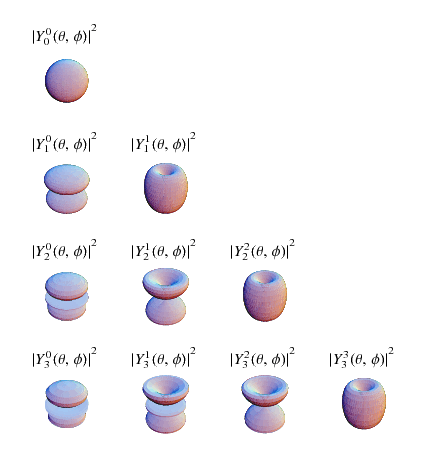
\includegraphics[width=6cm]{src/SphericalHarmonics.png}
\end{figure}
曲面上的点到原点的距离表示该方向上的$W$.
\begin{remark}
    $\theta$方向上的节点数为$l-\abs{m}$. $m \neq 0$时$\theta = 0,\pi$处总有$W=0$, 不计入节点.
\end{remark}
径向分布函数为
\[ W_{nl}\pare{r} = R_{nl}^2\pare{r}r^2. \]
这表示$r$处单位厚度球壳内电子出现的概率.
\begin{figure}[ht]
    \centering
    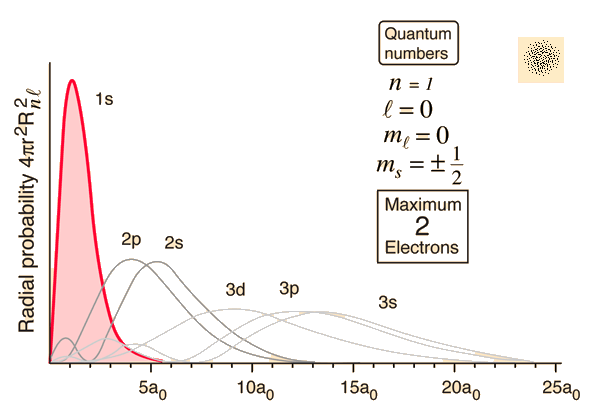
\includegraphics[width=8cm]{src/hy1s.png}
\end{figure}
\begin{remark}
    $r$方向上的节点数为$n-l-1$.
\end{remark}
\begin{cenum}
    \item 只有$l=0$的 \ce{s} 态才有$r=0$处$R$非零.
    \item $l=n-1$的态对应的最可几半径($W$最大者)为$r_m = n^2 a_0$.
    \item 平均半径
    \begin{align*}
        \expc{r}_{nlm} = \int_0^\infty \abs{R_{nl}\pare{r}}^2r^3\,\rd{r} = \frac{n^2 a_0}{Z}\curb{1 + \half \brac{1-\frac{l\pare{l+1}}{n^2}}}.
    \end{align*}
    \item 其它常用平均值有
    \begin{align*}
        \expc{r^2}_{nlm} &= \frac{n^4 a_0^2}{Z^2} \curb{1+\frac{3}{2}\brac{1 - \frac{l\pare{l+1} - 1/3}{n^2}}}, \\
        \expc{\rec{r}}_{nlm} &= \frac{Z}{a_0 n^2}, \\
        \expc{\rec{r^2}}_{nlm} &= \frac{Z^2}{a_0^2 n^3 \pare{l+1/2}}, \\
        \expc{\rec{r^3}}_{nlm} &= \frac{Z^3}{a_0^3 n^3 l\pare{l+1/2}\pare{l+1}}.
    \end{align*}
\end{cenum}

\paragraph{坐标空间和动量空间} % (fold)
\label{par:坐标空间和动量空间}

对于氢原子, $\displaystyle \psi\+_1s_\pare{r} = \rec{\sqrt{\pi}} e^{-r}$, Fourier变换可得$\displaystyle \phi\+_1s_\pare{p} = \frac{2^{3/2}}{\pi\pare{1+p^2}^2}$, 即$\abs{\phi\+_1s_\pare{p}}^2 = 8\pi^{-2} \pare{1+p^2}^{-4}$.
\par
从而空间概率密度的测量可以转化为动量概率密度的测量. 通过散射实验 \ce{e^- + A -> A^+ + e_1^- + e_2^-} 以及角动量守恒可得电子的动量分布.

% paragraph 坐标空间和动量空间 (end)

% subsubsection 氢原子的波函数 (end)

\subsubsection{量子数的物理意义} % (fold)
\label{ssub:量子数的物理意义}

\paragraph{主量子数} % (fold)
\label{par:主量子数}

主量子数直接关系到氢原子能级,
\begin{align*}
    n &= \frac{Ze^2}{4\pi\epsilon_0 \hbar} \pare{-\frac{m}{2E}}^{1/2}, \\
    E_n &= -\rec{2n^2} \pare{\frac{Ze^2}{4\pi\epsilon_0}}^2 \frac{m_e}{\hbar^2} \\
    &= -\half m_e \alpha^2 c^2 \frac{Z^2}{n^2},\quad n = 1,2,3,\cdots.
\end{align*}
对于给定的$n$, $l = 0,\cdots, n-1$, $m = 0,\pm 1,\cdots, \pm 1$, 一共有$n^2$个不同状态, 都具有相同的能量, 谓之$n^2$重简并的.

% paragraph 主量子数 (end)

\paragraph{角量子数} % (fold)
\label{par:角量子数}

轨道量子数$l$和角动量轨道大小有关系
\[ \hat{L}^2 Y_{lm}\pare{\theta,\varphi} = l\pare{l+1} \hbar^2 Y_{lm}\pare{\theta,\varphi}. \]
故$u_{nlm}$是$\hat{L}^2$的本征态, 相应的本征值为$l\pare{l+1}\hbar^2$. 即
\[ L = \sqrt{l\pare{l+1}}\hbar,\quad l = 0,1,2,\cdots, n-1. \]

% paragraph 角量子数 (end)

\paragraph{磁量子数} % (fold)
\label{par:磁量子数}

$\displaystyle Y_{lm}\pare{\theta,\varphi} = N_{lm} P_l^m \pare{\cos\theta} e^{im\varphi}$有
\[ \hat{L}_z Y_{lm}\pare{\theta,\varphi} = m\hbar Y_{lm}\pare{\theta,\varphi}. \]
从而$m$描述角动量的$z$分量,
\[ L_z = m\hbar,\quad m = 0,\pm 1,\cdots, \pm l. \]

% paragraph 磁量子数 (end)

\paragraph{角动量矢量} % (fold)
\label{par:角动量矢量}

$L$的大小是量子化的, $L_z$也是量子化的, 并且可以有确定本征值, 但$L_x$和$L_y$没有, 只有确定的期望值$\expc{L_x} = \expc{L_y} = 0$.

% paragraph 角动量矢量 (end)

\paragraph{空间取向量子化} % (fold)
\label{par:空间取向量子化}

$L = \sqrt{l\pare{l+1}}\hbar$, $L_z = m\hbar$, 从而$z$方向的取向是量子化的.

% paragraph 空间取向量子化 (end)

% subsubsection 量子数的物理意义 (end)

\subsubsection{氢原子波函数的宇称} % (fold)
\label{ssub:氢原子波函数的宇称}

设$\hat P$为宇称算符, 定义为$\hat P\varphi\pare{\+vr} = \hat P\varphi\pare{-\+vr}$, 则$\hat P^2 = \hat I$, 故本征值$\eta = \pm 1$.
\par
如果某个态$\eta = 1$, 则其满足空间反演对称, 体系具有偶宇称. 若$\eta = -1$, 则其满足空间反演反对称, 体系具有奇宇称.
\begin{ex}
    对于氢原子,
    \[ \hat P\brac{R\pare{r}Y\pare{\theta,\phi}} = R\pare{r}Y\pare{\pi - \theta,\phi + \pi} = R\pare{r}\pare{-1}^lY_{lm}\pare{\theta,\phi}. \]
    因此波函数的宇称取决于$l$, $l$的奇偶性决定了宇称的奇偶性.
\end{ex}

% subsubsection 氢原子波函数的宇称 (end)

\subsubsection{原子定态} % (fold)
\label{ssub:原子定态}

定态下电子的概率分布不随时间变化, 故不发生辐射.

% subsubsection 原子定态 (end)

\subsubsection{电偶极跃迁} % (fold)
\label{ssub:电偶极跃迁}

对于经典的电偶极震荡, 电偶极矩为
\[ \+vp = \pare{-e}\+vr = \pare{-e}\+vr_0 \sin \omega t = \+vp_0 \sin \omega t, \]
平均辐射功率为
\[ \overbar{P} = \frac{\omega^4}{12\pi\epsilon_0 c^3}\abs{\+vp_0}^2. \]
跃迁速率
\[ \lambda = \frac{\overbar{P}}{h\nu} = \frac{\omega^3}{6\epsilon_0 hc^2}\abs{\+vp_0}^2. \]
\par
在量子力学情形下, 跃迁$\displaystyle \psi_i \mapsto \varphi_f$, 跃迁过程中处于叠加态$\psi = c_i \psi_i + c_f \psi_f$.
\[ \expc{\+vp} = \expc{\pare{-e}\+vr} = \iiint \rd{V}\, \psi^* \pare{-e} \+vr\psi. \]
由
\[ \psi^* \psi = c^*_i c_f \psi^*_i \psi_f + c^*_f f_f u^*f u_f + c^*_i c_f u^*_i u_f e^{i\pare{E_i - E_f}t/\hbar} + c_i c^*_f e^{-i\pare{E_i - E_f}t/\hbar}. \]
可得
\[ \expc{p} = -\expc{e\+vr} = \iiint\rd{V}\, \psi^*_f \pare{-e\+vr}\psi_i. \]
跃迁速率
\[ \lambda_{fi} = \frac{\omega^3}{6\epsilon_0 hc^3}\abs{\expc{\+vp}}^2 = \frac{\omega^3}{6\epsilon_0 hc^3} \abs{\iiint \rd{V}\, u^*_f \pare{-e\+vr}u_i}^2. \]
跃迁的发生要求
\[ \lambda_{fi} \propto \abs{\iiint \rd{V}\, u^*_{n'l'm'}u_{nlm}}^2 \neq 0. \]
可得跃迁的选择定则.
\begin{resume}
    选择定则
    \begin{align*}
        \Delta n &= n' - n = \forall,\\
        \Delta l &= l' - l = \pm 1, \\
        \Delta m &= m' - m = 0,\pm 1.
    \end{align*}
\end{resume}
\begin{ex}
    氢原子中 \ce{s} 态到 \ce{s} 态的跃迁不发生.
\end{ex}

% subsubsection 电偶极跃迁 (end)

\subsubsection{辐射} % (fold)
\label{ssub:辐射}

\begin{cenum}
    \item 受激辐射: 吸收一光子, 发射二光子.
    \item 吸收: 吸收一光子.
    \item 自发辐射: 发射一光子.
\end{cenum}
假设原子只有两个能级, 大量这样二能级的原子处于辐射场中, 温度$T$下达到平衡. 辐射场在频率$\pare{\omega,\rd{\omega}}$的能量密度为$I\pare{\omega}\,\rd{\omega}$.
\begin{cenum}
    \item 吸收的跃迁概率$B_{if}I\pare{\omega}$, 吸收系数$B_{if}$.
    \item 受激辐射的跃迁概率$B_{fi}I\pare{\omega}$, 受激辐射系数$B_{fi}$.
    \item 自发辐射的跃迁概率$A_{fi}$, 自发辐射系数$A_{fi}$.
\end{cenum}
温度$T$下达到平衡, 激发的原子数$\propto B_{if}I\pare{\omega}N_f$, 退激发的原子数$\propto \pare{A_{fi} B_{fi}I\pare{\omega}}N_i$. 达到平衡时, 激发的原子与退激发的原子数相等,
\[ \pare{A_{fi} + B_{fi}I\pare{\omega}}N_i = B_{if}I\pare{\omega}N_f \Rightarrow \frac{N_i}{N_f} = \frac{B_{if}I\pare{\omega}}{A_{fi} + B_{fi}I\pare{\omega}}. \]
另一方面, 处于不同能级的原子数服从Boltzmann统计分布
\begin{align*}
    \frac{N_i}{N_f} &= \exp\pare{-\frac{E_i - E_f}{k_BT}} = \exp\pare{-\frac{\hbar\omega}{k_BT}}, \\
    \exp\pare{-\frac{\hbar\omega}{k_BT}} &= \frac{B_{if}I\pare{\omega}}{A_{fi} + B_{fi} I\pare{\omega}}, \\
    I\pare{\omega} &= \frac{A_{fi}}{B_{if}} \rec{\displaystyle \exp\pare{\frac{\hbar\omega}{k_BT}} - \frac{B_{fi}}{B_{if}}}.
\end{align*}
与Planck黑体辐射公式比对,
\begin{align*}
    I\pare{\omega} &= \frac{\hbar\omega^3}{\pi^2 c^3} \rec{\displaystyle \exp\pare{\frac{\hbar\omega}{k_BT}} - 1} = \frac{A_{fi}}{B_{if}}\rec{\displaystyle \exp\pare{\frac{\hbar\omega}{k_BT}} - \frac{B_{fi}}{B_{if}}},\\
    B_{fi} &= B_{if},\quad A_{fi} = \frac{\hbar \omega^3}{\pi^2 c^3}B_{fi}, \\
    B_{fi} &= B_{if} = \lambda_{fi} = \frac{\omega^3}{6\epsilon_0 hc^3} \abs{\expc{\+vp}}^2 = \frac{\omega^3}{6\epsilon_0 hc^3}\abs{\iiint \rd{V}\, u^*_f \pare{-e\+vr} u_i}^2.
\end{align*}

% subsubsection 辐射 (end)

\subsubsection{能级的平均寿命} % (fold)
\label{ssub:能级的平均寿命}

没有外界辐射场, 原子间无碰撞无辐射跃迁时, 处于激发态的原子仍可以通过自发辐射退激发. 每个原子的退激发独立进行, 激发态存在的时间长短随机, 退激发速率确定,
\[ \rd{N_i} = -A_{fi}N_i \,\rd{t} \Rightarrow N_i\pare{t} = N_{i0} \exp\pare{-A_{fi}t}. \]
相应的平均寿命为
\[ \tau = \rec{N_{i0}} \int_{N_{i0}}^0 t\pare{-\rd{N_i}} = \rec{A_{fi}}. \]
衰变公式可以写为
\[ N_i\pare{t} = N_{i0}e^{-t/\tau},\quad N_i\pare{\tau} = N_{i0}/e. \]

% subsubsection 能级的平均寿命 (end)

\subsubsection{能级自然宽度} % (fold)
\label{ssub:能级自然宽度}

能量和时间有不确定关系
\[ \Gamma \tau = \hbar. \]
$\Gamma$为能级宽度. 原子分子的低激发态的能级寿命一般在$10^{-8}\sim 10^{-9}\SI{}{\second}$, 相应的能级宽度$10^{-8}\sim 10^{-7}\SI{}{\eV}$. 对于稳定的基态, $\tau = \infty$, $\Gamma = 0$.

% subsubsection 能级自然宽度 (end)

\subsubsection{原子光谱} % (fold)
\label{ssub:原子光谱}

\begin{cenum}
    \item 满足电偶极矩的选择定则.
    \item $\omega = \pare{E_i - E_f}/\hbar$.
    \item 谱线强度$I \propto N_i \lambda_{fi}$.
    \item 谱线宽度: 自然宽度, Doppler展宽, 仪器分辨率.
\end{cenum}

% subsubsection 原子光谱 (end)

% subsection 氢原子 (end)

% section 量子力学初步 (end)

\end{document}
